%# -*- coding: utf-8-unix -*-
%%==================================================
%% chapter1.tex for SJTU Master Thesis
%%==================================================

\chapter{基于农业物联网的智能温室架构}
\label{chapter:IoT Architecture}

\section{农业物联网简介}
	\subsection{物联网概念}
	物联网的概念最早来源于比尔·盖茨于1995年发表的《The Road Ahead(未来之路)》一书中所提及的Internet of Things的概念\supercite{TheRoadAhead},但是受限于当时的网络技术、传感器技术和智能硬件技术,并没有引起广泛的关注和重视\supercite{NongYeWuLianWang}。直到1999年,麻省理工学院自动识别中心(Auto-ID Center)率先提出“物联网”的概念,主要建立在物品编码、RFID技术和互联网的基础上\supercite{ZiJiDongShouIoT}。2005年国际电信联盟(International Telecommunication Union,ITU)在《ITU Internet Report 2005: The Internet of Things》中正式提出了“物联网”的概念\supercite{2005ITU,NongYeWuLianWang}。
	
	为了解释物联网这一概念,首先要了解这个词是如何被创造的,物联网之父Kevin Ashton曾指出,互联网中的大部分数据都是通过人为的控制进入系统中的,在系统中,人所充当的角色无非是一种效率低下、易出错、对数据的数量和质量有所限制的路由器,并在一定的情况下可以对数据进行解释和修正,但是从另一个角度如果系统如果能够抛开人的限制直接连接到互联网,通过传感器获取现实世界的数据并对现实世界进行一定的控制,这样会变得更加高效、丰富和准确。物联网也即是万物相连的互联网,我们连接物体所获得的一切都是由互联网和物体自身控制,而非人\supercite{LearningIoT}。因此,物联网是建立在互联网的基础之上的,是互联网的延伸和拓展,而信息的获取和交换从人为控制扩展到了物和物之间自主进行。我们可以用一个非常简单的组成关系来描述物联网的基本构成,如\ref{fig:CompositionIoT}所示。
	\begin{figure}[!htp]
  		\centering
 		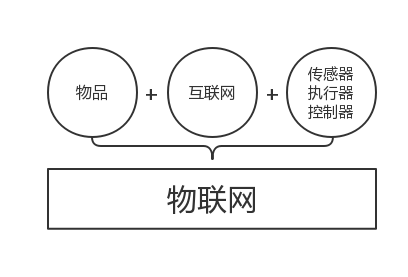
\includegraphics[width=0.5\textwidth]{chapter1/CompositionIoT.png}
  		\bicaption[fig:CompositionIoT]{物联网的基本构成}{物联网的基本构成}{Fig}{Composition of the Internet of Things}
	\end{figure}
	
	\subsection{物联网的特征及内涵}
	根据物联网的概念、物联网和互联网的联系与区别,结合国内外专家的阐述,物联网具有如下的特征和内涵:
	\begin{enumerate}
  			\item 物联网广泛运用了各种感知技术。物联网系统中包含大量不同类型的传感器,每个传感器都担任着连接万物的使命,连续不断的捕获和更新外界的实时数据。
  			\item 互联网是物联网的基础,物联网是建立在互联网上的网络,是互联网的延伸。物联网并不是一种全新的信息传递网络,其核心和基础仍是互联网,通过各种有线或者无线网络接入互联网进行物体信息的实时传递,实现物与物、人与物的实时交互,最终达到为人服务的目的。
  			\item 物联网自身也是一个智能系统,它不仅可以通过传感器获取数据,同样也具备智能分析处理的能力,对数据进行清洗筛选得到有意义的数据,然后通过控制器和执行器对物体进行智能控制。
  			\item 物联网即是未来的互联网。狭义上无论是否接入互联网,只要实现物与物通过传感网络相连的网络都属于物联网范畴,但是我们希望实现的不仅仅是物与物的局部信息传递,而是最终要实现所有的人和世间万物的互连互通,这也与未来的互联网的发展趋势是一致的。
	\end{enumerate}
	
	\subsection{物联网在农业中的应用}
	物联网被称为是继计算机、互联网之后,第三次世界范围内的信息产业浪潮\supercite{LingZhihao2010}。“十三五”规划纲要也指出要加快构建高速、移动、安全、泛在的新一代信息基础设施,推进信息网络技术广泛运用,形成万物互联、人机交互、天地一体的网络空间,推进物联网感知设施规划布局,发展物联网开环应用。同时指出要推进农业现代化和信息化建设,推动信息技术与农业生产管理、经营管理、市场流通、资源环境等融合;实施农业物联网区域试验工程,推进农业物联网应用,提高农业智能化和精准化水平;推进农业大数据应用,增强农业综合信息服务能力。物联网技术的发展为实现农业的现代化、智能化、信息化和精准化带来新的解决方案和发展机遇。
	
	目前,物联网技术在工业领域已经得到了较为广泛的应用,农业领域的物联网应用还处在研究发展阶段。近十年来,欧美等发达国家相机开展了农业物联网的相关研究,实现了农业生产管理、农业资源利用和精准农业的实践推广,推动了农业物联网的发展。我国也在农业物联网相关方面开展了积极的研究工作,主要实现农业生产环境、农业资源、生产和流通过程的信息获取和通信,形成产前合理规划提高资源利用率,产中现代化管理提高生产效率、安全生产、节约成本提高效益,产后高效流通和安全溯源的农业物联网一条龙解决方案,但是产品多处于试验阶段,产品的稳定性、可靠性、低功耗等性能参数上与国际领先的产品还存在一定的差距。因此我国的农业物联网开发和研究工作还有很大的发展空间\supercite{ChenWei2013}。
	
	\subsection{农业物联网的特点}
	农业的生产环境和工业环境相比,有其自身的特点和限制,这也决定了农业物联网所处的物理环境和网络条件与工业物联网有着本质的区别。因此农业物联网有其自己的特点和特殊的需求,主要有如下几点:
	\begin{enumerate}
  			\item 农业生产的单位收益不高,农田面积往往较大,投入成本有限,此外,大面积在农田内布置传感器测点会给农业作业,尤其是农业机械化作业带来干扰,这就决定了农业物联网中不可能密集布置传感器测点。因此,农业物联网在大规模农田中应用时,往往布置稀疏的传感器测点,即通常情况下,根据实际的生产管理需要和生产环境的实际情况将农田划分为若干个小区域,近似地认为各个区域内环境相同,在每个区域内布置一套传感器设备。这就要求农业物联网具有远距离传输和可灵活扩展的能力。
  			\item 农业物联网工作环境往往面积较大且地形复杂,不易于值守,也无市电供电。因此,在要求各节点具有远距离传输能力的同时还要求功耗尽量小,能够依靠环境能源实现长期不间断的工作。
  			\item 农业生产环境恶劣,设备经常长时间工作在高温、高湿、低温等极端环境下,且在进行无线通信时易受作物植被的干扰,这就对农业物联网设备的稳定性、可靠性、自诊断和免维护能力提出了要求。
	\end{enumerate}

\section{系统整体架构设计}
	\subsection{物联网层次定义}
	根据一般的物联网架构层次定义\supercite{Yu2011Research,LiuQiang2010},物联网可分为感知层、网络层和应用层三层结构\supercite{HanYi2016A,WangHuaiyu2015},如\ref{fig:ArchitectureIoT}所示。
	\begin{figure}[!htp]
  		\centering
 		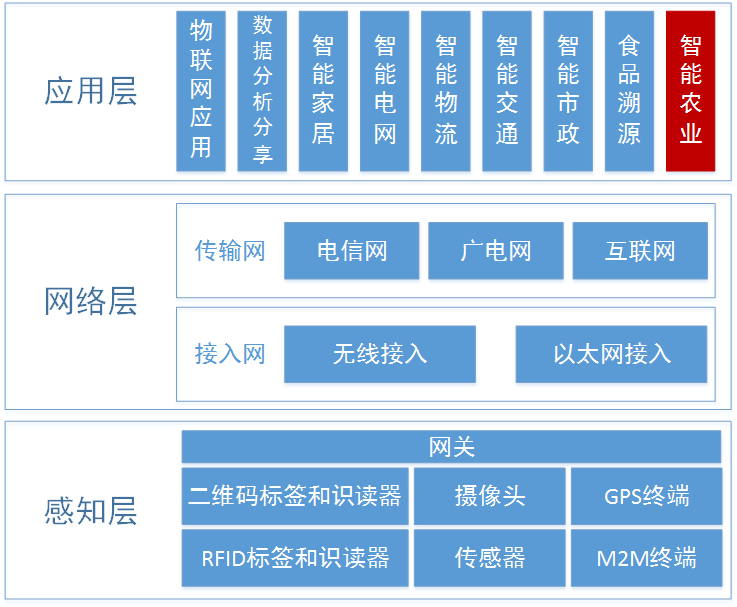
\includegraphics[width=0.8\textwidth]{chapter1/ArchitectureIoT.png}
  		\bicaption[fig:ArchitectureIoT]{物联网层次架构}{物联网层次架构}{Fig}{Architecture of the Internet of Things}
	\end{figure}
	感知层是物联网的核心部分,位于物联网三层结构的最底层,是信息采集的关键部分,是架设在人类世界和物理世界之间的桥梁,主要负责物联网系统的“感知”,相当于人类五官的功能,包含各种感应器件和感应器组成的网络两部分,可以对物体的各类属性和环境状态等数据信息进行动态感知、快速识别和信息采集。该层的核心技术包括射频技术、新兴传感技术、无线网络组网技术、现场总线控制技术等,涉及的核心产品包括二维码标签和识读器、RFID标签和读写器、摄像头、GPS终端、传感器、M2M终端、各类网关等。
	
	网络层是物联网的枢纽部分,位于物联网三层结构中的第二层,是信息传输的重要部分,其功能为“传送”,即通过通信网络进行信息传输。网络层作为纽带连接着感知层和应用层,它由各种私有网络、互联网、有线和无线通信网等组成,相当于人的神经中枢系统,负责将感知层获取的信息,安全可靠地传输到应用层,然后根据不同的应用需求进行信息处理。网络层包含接入网和传输网,分别实现接入功能和传输功能。传输网由公网与专网组成,典型传输网络包括电信网、广电网、互联网等;接入网包括无线接入、以太网接入等各类接入方式,实现底层的传感器网络、RFID网络的接入。物联网的网络层基本上综合了已有的全部网络形式,来构建更加广泛的“互联”。
	
	应用层位于物联网三层结构中的最顶层,主要负责处理各种信息处理。应用层与最低层的感知层一起,是物联网的显著特征和核心所在,应用层可以对感知层采集数据进行计算、处理和知识挖掘,从而实现对物理世界的实时控制、精确管理和科学决策。目前,其核心功能主要围绕数据的管理与处理,以及数据与各行业应用相结合。从结构上划分,物联网应用层主要包括物联网中间件、物联网应用和云计算。从物联网三层结构的发展来看,网络层已经非常成熟,感知层的发展也非常迅速,而应用层不管是从受到的重视程度还是实现的技术成果上,以前都落后于其他两个层面。但因为应用层可以为用户提供具体服务,是与我们最紧密相关的,因此应用层的未来发展潜力很大。
	
	\subsection{智能温室整体架构设计}
	根据一般物联网架构层次定义和农业生产的特殊需求,本文基于农业物联网的智能温室系统自底向上划分为感知控制层、网络传输层和应用层,另外为了兼容各类终端设备接入添加了终端接入层\supercite{WangHuaiyu2015},如\ref{fig:System}所示。
		\begin{figure}[!htp]
  			\centering
 			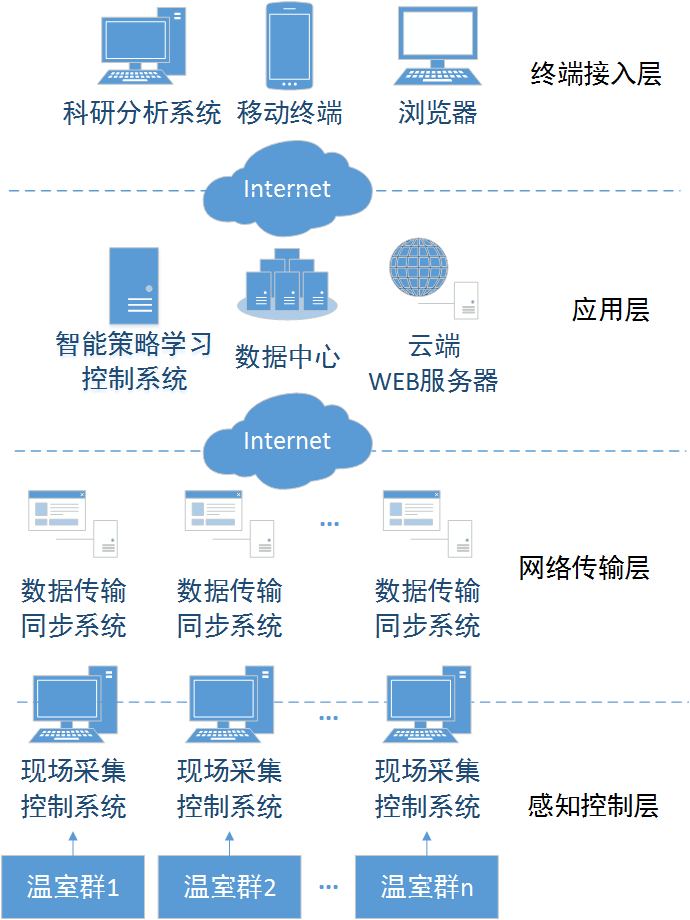
\includegraphics[width=0.6\textwidth]{chapter1/ArchitectureSystem.png}
  			\bicaption[fig:System]{智能温室系统整体架构}{智能温室系统整体架构}{Fig}{Architecture of the intelligent greenhouse system.}
		\end{figure}
		
\section{感知控制层}
感知控制层主要用于获取需要监测及用于控制的各类温室环境参数数据,已经对温室现场的作动器进行控制以达到控制温室内环境参数的目的。本层通过现场采集控制系统实现,其总体设计如\ref{fig:Sensing}所示。针对农业特殊的生产环境,本层适合使用可靠性高、稳定性强、灵活性大、易于扩展的传感器网络采集温室环境参数数据,如基于RS485总线的传感器网络、基于ZigBee的无线传感器网络等。
		\begin{figure}[!htp]
  			\centering
 			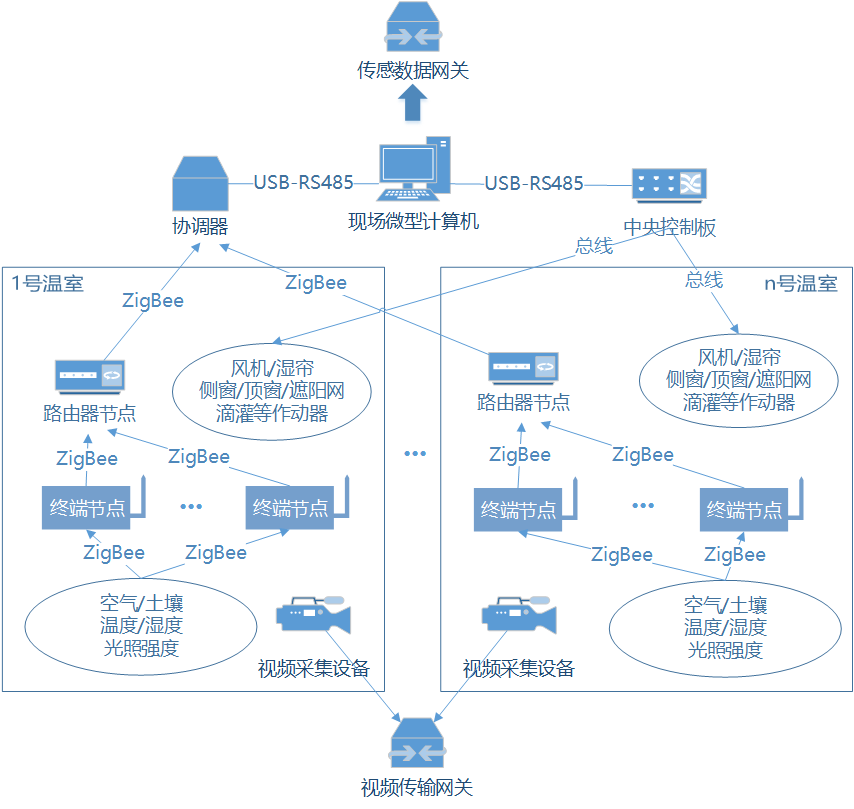
\includegraphics[width=0.8\textwidth]{chapter1/sensing.png}
  			\bicaption[fig:Sensing]{智能温室系统整体架构}{智能温室系统整体架构}{Fig}{Architecture of the intelligent greenhouse system.}
		\end{figure}

监测到当前温室环境后,系统需要通过控制温室内作动器的动作对温室内的环境加以控制,从而达到让温室环境更加适宜温室内作物生长的目的。因此本层还包括用于控制温室内作动器的中央控制板。为降低成本的同时提高设备的可靠性,本系统适合采用嵌入式计算机提供现场计算服务,同时兼用作网关服务,如基于ARM的微型计算机等。另外,为了增加对温室内环境的直观感知,本层添加了图像采集模块,包括图像采集设备和图像传输网关,该模块可在需要视频或图像监测的温室内使用。
\section{网络传输层}

\section{应用层}

\section{终端接入层}
 
